\section{Informations sur les documents contenus dans la présente annexe}
Les sections suivantes contiennent les rapports intermédiaires fournis à notre maître de stage et au autres membres du projet au cours du \gls{project_papud}.

\subsection{Format d'origine, transcription et contenu des rapports}
Pour les mêmes raisons que pour l'annexe précédente (décrite dans la \autoref{report_infos}), les documents présentés dans cette annexe ont été rédigés en anglais, au format \gls{git_md}; les versions présentées ici sont des transcriptions aussi fidèles que possible de ces documents.

\newpage
\begin{report}{Informations générales}
	\section*{General information}

\subsection{Corpus}

\subsubsection{firsttest}

\paragraph{Baseline accuracy}

True baseline accuracy (for char \lstinline!-!): training 0.443; valid
0.414; test 0.423

\begin{longtable}[]{@{}llll@{}}
\hline
char & training & valid & test\tabularnewline
\hline
\endhead
\lstinline!-! & \textbf{0.443} & \textbf{0.414} & \textbf{0.423}\tabularnewline
\lstinline! ! & 0.064&0.067&0.063\tabularnewline
\lstinline!a! & 0.021&0.022&0.023\tabularnewline
\lstinline!0! & 0.015&0.013&0.011\tabularnewline
\lstinline!<unk>! & 0.0&0.0&0.0\tabularnewline
\hline
\end{longtable}

\subsection{Grid-5000}

To develop and train the model, we are using Grid-5000 computers
clusters. For specific information on Grid-5000, see
\href{https://www.grid5000.fr/}{https://www.grid5000.fr/}.

\subsubsection{GPU-equipped nodes}

Due to the properties of neural networks models, it is really efficient
to use GPUs to train them.

Here are the main GPU-equipped nodes of Grid-5000:

\begin{longtable}[]{@{}rcrrcc@{}}
\hline
Nodes & GPU & Graphical memory & RAM & Production & CUDA\tabularnewline
\hline
\endhead
graphique-1 & 2 x Nvidia Titan Black & 2 x 6GB & 64GB & X &
2880\tabularnewline
graphique-2/6 & 2 x Nvidia GTX 980 & 2 x 4GB & 64GB & X &
2048\tabularnewline
graphite-1/4 & Intel Xeon Phi 7120P & 16GB & 256GB & & ?\tabularnewline
grele-1/14 & 2 x Nvidia GTX 1080 Ti & 2 x 11GB & 128GB & X &
3584\tabularnewline
grimani-1/6 & 2 x Nvidia Tesla K40M & 2 x 12GB & 64GB & X &
2880\tabularnewline
\hline
\end{longtable}

\section*{{[}NOT TESTED YET{]} Model conversion}

See 
\href{https://github.com/ysh329/deep-learning-model-convertor}{https://github.com/ysh329/deep-learning-model-convertor}

\end{report}
\begin{report}{Résultats de l'implémentation basique}
	\section*{Results of the basic implementation of the
model}

2018/07/09 - SYNALP - Esteban MARQUER

\subsection{Paradigm}

The test is run on a minimal number of epoch (10), with a minimal model.

The training algorithm used is an example by example training.

\subsubsection{Model architecture}

The model is a line by line predictive model, composed of: - a character
embedding layer; - a pooling layer; - a linear layer; - an output layer.

The output of the model is a probability distribution over known
characters for every character of the predicted line.

\subsection{Results}

\subsubsection{GPU memory usage}

As expected from the model architecture, GPU memory usage is constant.

\begin{figure}[ht]
\centering
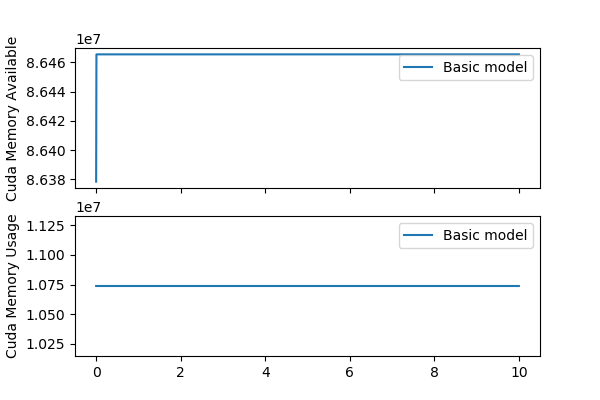
\includegraphics{parts/appendix/reports-papud/2018_07_09-Basic_implementation_results/memory.png}
\caption{memory usage}
\end{figure}

\subsubsection{Computation time}

\subsubsection{Loss and accuracy}

The loss used is cross-entropy loss, a character per character
negative-log-likelihood loss over the soft-maxed distribution.

Overall, the loss gives a score to the prediction of the model, by
comparing the target character and a distribution of probabilities for
each character. If the probability for the target character is high and
other character low, the model does a good prediction of the character,
and the score given is low. The closer the score is to 0, the better it
is. The scores of each characters is averaged, producing a global loss
over the line.

Accuracy is a percentage. The closer to 100 \% the better. As the loss
is bound by 0 and +Infinity, and the closer to 0 the better, a correct
transformation to accuracy could be: \lstinline!exp(-loss)! for an
accuracy between 0 and 1.

\begin{figure}[ht]
\centering
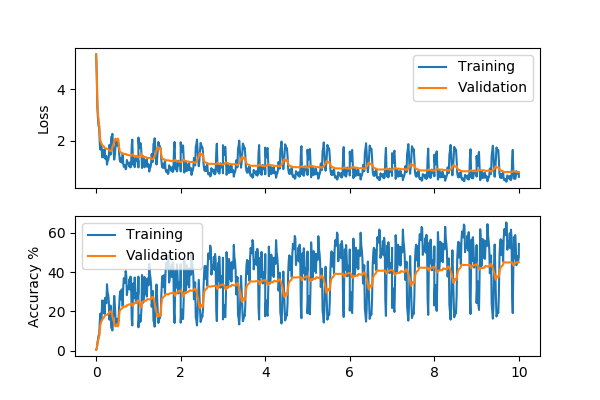
\includegraphics{parts/appendix/reports-papud/2018_07_09-Basic_implementation_results/loss.png}
\caption{loss}
\end{figure}

The small spike recurrently appearing in the loss and accuracy is most
likely due to a noisy part of the corpus (around the middle of the
corpus) causing the model to learn wrongly on those specific examples.

The best precision obtained at the end of 10 epochs is 50\%,
corresponding to a loss of about 0.7.

\subsection{Improvements and next
steps}

\subsubsection{Mini-batch}

Currently, the models learn one example at a time, meaning it computes
the result for a line of input, compares it to the target, and updates
weights. A common algorithm is the mini-batch algorithm, computing
simultaneously a set of examples, their loss compared to the target, and
updates the weights of the model all at once for the whole set of
examples.

This algorithm speeds-up training while making the most of the GPU.

\subsubsection{Dynamic corpus}

While with the current corpus there is no real problem in storing the
whole corpus in the memory, the future corpus will be over 400GB of
text. It is necessary to replace the current method by a dynamic loading
and transformation of the parts of the corpus currently used by the
model. An ideal solution would be to read the target data directly from
the archive containing the corpus.

\end{report}
\begin{report}{Paquets (\foreign{batchs}) simultanés}
\section*{Increasing the number of simultaneous
examples}

2018/07/10 - SYNALP - Esteban MARQUER

\subsection{Paradigm}

The test is run on a small number of epoch (20), with a minimal model
and a new training algorithm.

The training algorithm used is a \textbf{mini-batch training}, meaning
we compute the output for multiple examples all at once, we compute an
averaged loss over those examples, and we update the model.

The potential effects of this algorithm are:
\begin{itemize}
\item an increase of GPU memory usage, as computations are done on larger data;
\item a decrease of computation time, with the number of computations reduced;
\item a smother training loss, because it is averaged over multiple examples;
\item avoidance of some local minima.
\end{itemize}

A second test with random batch-size between 1 and 1000 was done on 50
epoch, to evaluate the effect of the batch size and find an optimum.

\subsection{Results}

\subsubsection{GPU memory usage}

As more examples are fed to the model, there is a very slight increase
in GPU memory usage: 0.013e7 B, corresponding to 127kiB (this amount is
negligible with more than 10GiB available and a current usage of about
10MiB).

\textbf{Conclusion:} increasing the number of simultaneous examples has
no substantial downsides memory-wise.

\begin{figure}[ht]
\centering
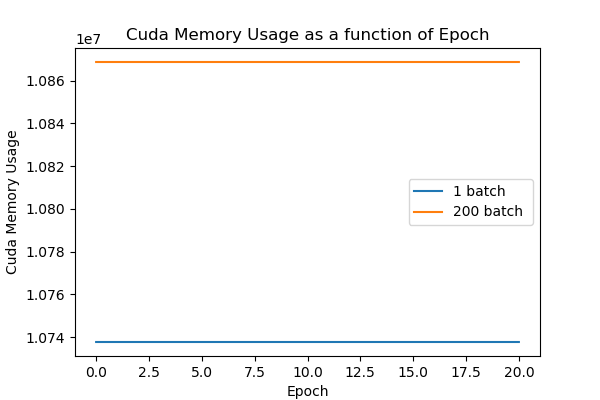
\includegraphics{parts/appendix/reports-papud/2018_07_11-Simultaneous_batches/memory.png}
\caption{memory usage}
\end{figure}

\subsubsection{Loss and accuracy}

As loss is averaged on multiple examples, it should be smoother. But,
probably because the number of simultaneous examples is too small, there
is no noticeable change of loss, with the curves superposed.

\textbf{Conclusion:} increasing the number of simultaneous examples has
no substantial effect loss-wise.

\begin{longtable}[]{@{}lll@{}}
\hline
Train. + Valid. & Training only & Validation only\tabularnewline
\hline
\endhead
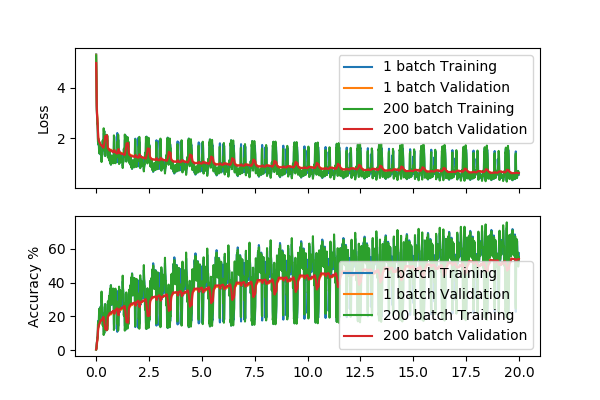
\includegraphics[width=.3\textwidth]{parts/appendix/reports-papud/2018_07_11-Simultaneous_batches/loss.png} & 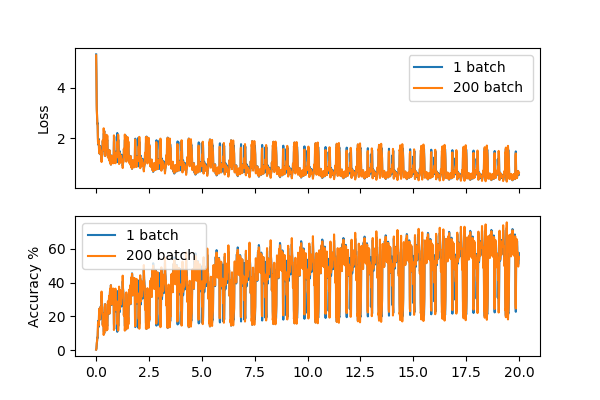
\includegraphics[width=.3\textwidth]{parts/appendix/reports-papud/2018_07_11-Simultaneous_batches/loss_train.png} &
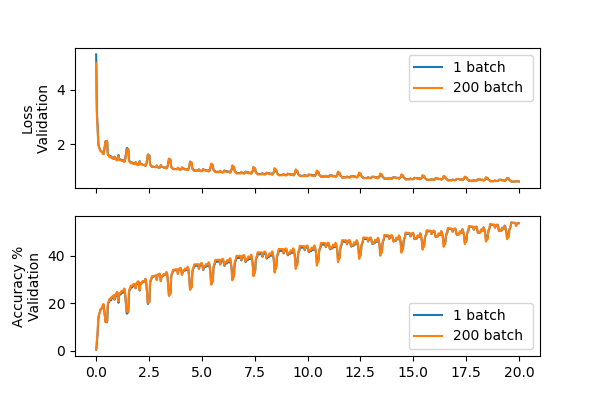
\includegraphics[width=.3\textwidth]{parts/appendix/reports-papud/2018_07_11-Simultaneous_batches/loss_valid.png}\tabularnewline
\hline
\end{longtable}

\subsubsection{Computation time}

The computations done on GPU benefit from grouping similar operations.
By computing multiple examples together, we can use this property to
speed up training. Moreover, retro-propagation and model updates are
less frequent, reducing computational load and training time.

The best-case time allow an improvement from 10ms to less than 2ms per
\textbf{training} sequence with a batch-size of 50, and the worst-case
one allow 4ms per training sequence with a batch-size of 200.

A small gain can be achieved on \textbf{validation} time by increasing
batch size over 50, but increasing it more has no effect.

\textbf{Conclusion:} increasing the number of simultaneous examples
leads to a notable improvement of computation time.

\begin{longtable}[]{@{}ll@{}}
\hline
Training time & Validation time\tabularnewline
\hline
\endhead
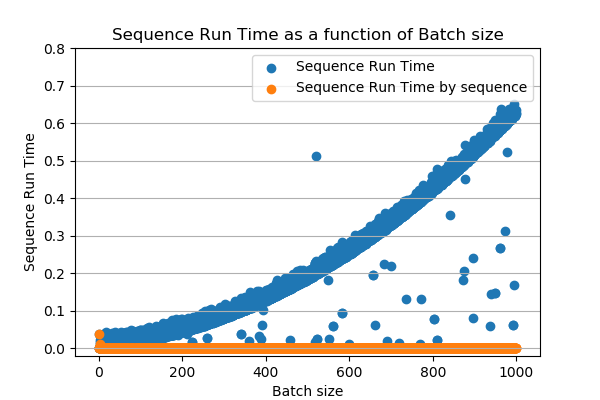
\includegraphics[width=.45\textwidth]{parts/appendix/reports-papud/2018_07_11-Simultaneous_batches/sequence_time.png} &
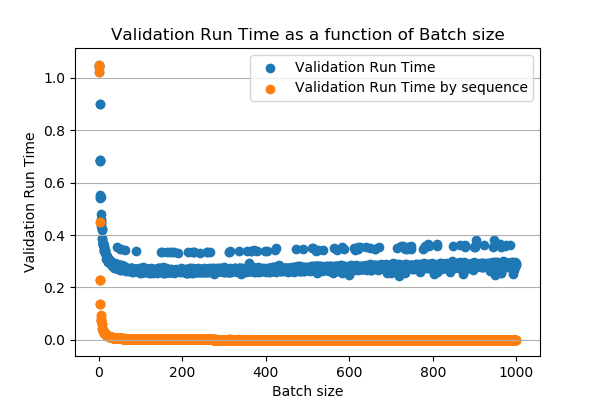
\includegraphics[width=.45\textwidth]{parts/appendix/reports-papud/2018_07_11-Simultaneous_batches/valid_time.png}\tabularnewline
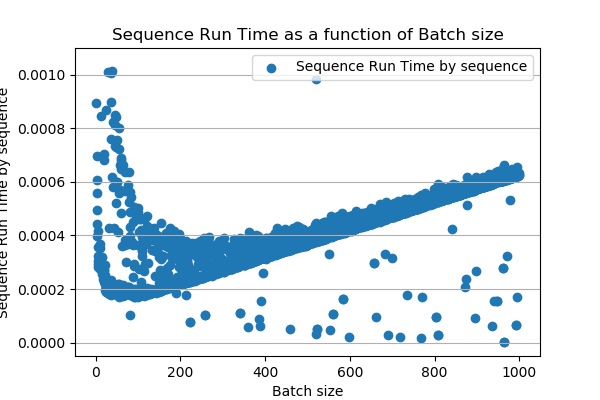
\includegraphics[width=.45\textwidth]{parts/appendix/reports-papud/2018_07_11-Simultaneous_batches/sequence_time_.png} &
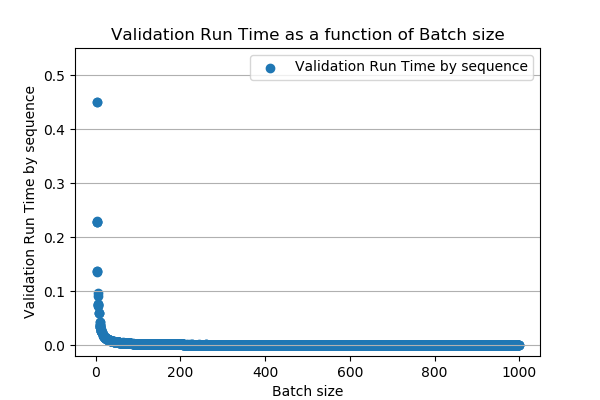
\includegraphics[width=.45\textwidth]{parts/appendix/reports-papud/2018_07_11-Simultaneous_batches/valid_time_.png}\tabularnewline
\hline
\end{longtable}

\subsection{Conclusion}

Even if there is no improvement of loss or memory, the gain in
computation time is enough to accept this algorithm.

The ideal batch-size (with the current node ``grele'') is between 50 and
200. In future works, a batch-size of 200 will be used, as it present
the best worst- and best-case time performances.

\subsection{Improvements and next
steps}

\subsubsection{Dynamic corpus}

The dynamic corpus implementation is ready (except small details) and
working, only integration is left.

\paragraph{Buffer size}

The dynamic corpus can use a buffer, and the size of this buffer must be
at least the size of the batch. It will be necessary to test which size
is optimal. An optimal buffer has the minimal size to make computation
time over the buffer size only slightly higher than pre-loading time. It
allows training to continue without interruption, while maintaining a
low memory usage.

\end{report}
\begin{report}{Analyse du pic de performance}
\section*{Performance spike analysis}

2018/07/18 - SYNALP - Esteban MARQUER

\subsection{Problem}

During training, a big performance spike appeared periodically. It is
necessary to know why this spike appeared.

The different parts of the spike are:
\begin{itemize}
\item from line 24545 to line 31558 (35\% to 45\% of the corpus): the increase of the BPC;
\item from line 31558 to line 36468 (45\% to 52\% of the corpus): a stable part at a high value;
\item from line 36468 to line 38572 (52\% to 55\% of the corpus): the decrease of the BPC.
\end{itemize}

\begin{longtable}[]{@{}ll@{}}
\hline
Loss of 1 epoch (first epoch) & Zoom on spike\tabularnewline
\hline
\endhead
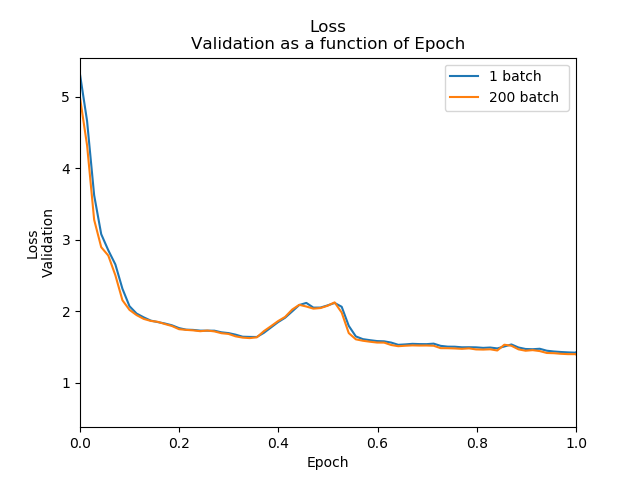
\includegraphics[width=.45\textwidth]{parts/appendix/reports-papud/2018_07_18-Performance_spike_analysis/loss_valid.png} &
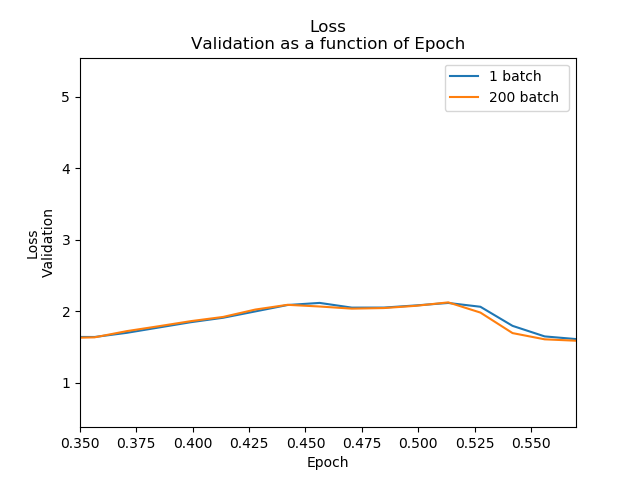
\includegraphics[width=.45\textwidth]{parts/appendix/reports-papud/2018_07_18-Performance_spike_analysis/loss_valid_part.png}\tabularnewline
\hline
\end{longtable}

\subsection{Analysis}

By extracting the parts of the corpus corresponding to the parts of the
spike, and scrolling through them, some recurrent elements appear: -
lines beginning by \lstinline!kern!, more specifically
\lstinline!kern info! and \lstinline!kern debug!; - lines containing a
memory address, like \lstinline!0x91ffffff!, \lstinline!0x0093! and
\lstinline!00000000fed18000!, or an error code like \lstinline!0x0100!,
- lines beginning by \lstinline!daemon!, more specifically
\lstinline!daemon err!;

The most interesting part of the spike is the increase of the BPC, were
the performance deteriorate.

Given the repartition and percentages (see the next two sub-sections),
the most likely causes for the spikes are:
\begin{itemize}
\item the memory address and
hexadecimal codes;
\item the kernel messages (very repetitive, and
containing memory address and hexadecimal codes).
\end{itemize}

\paragraph{Examples of Kernel
messages}

\begin{lstlisting}
kern info kernel ACPI: LAPIC (acpi_id[0x00] lapic_id[0x00] enabled)
kern info kernel ACPI: LAPIC (acpi_id[0x02] lapic_id[0x02] enabled)
kern info kernel ACPI: LAPIC (acpi_id[0x04] lapic_id[0x04] enabled)
kern info kernel ACPI: LAPIC (acpi_id[0x06] lapic_id[0x06] enabled)
kern info kernel ACPI: LAPIC (acpi_id[0x08] lapic_id[0x08] enabled)
\end{lstlisting}

\subsubsection{Repartition of match in the
corpus}

The ``localisation bars'' (vertical blue lines) delimit to the different
parts of the spike.

\begin{longtable}[]{@{}lll@{}}
\hline
Type of element & With localisation bars & With
subcategories\tabularnewline
\hline
\endhead
Memory addresses & 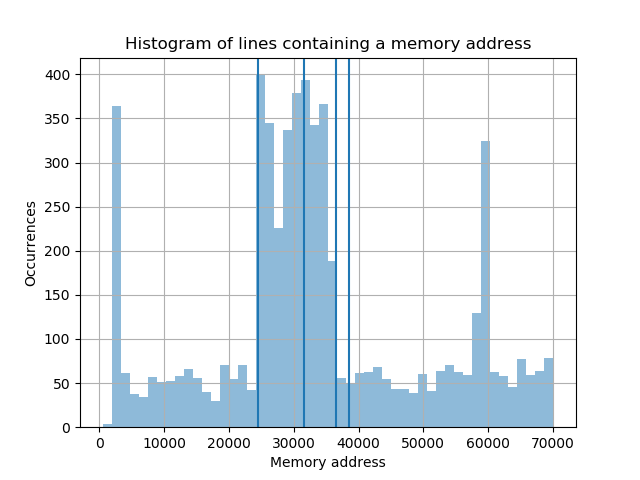
\includegraphics[width=.25\textwidth]{parts/appendix/reports-papud/2018_07_18-Performance_spike_analysis/memory_.png} &
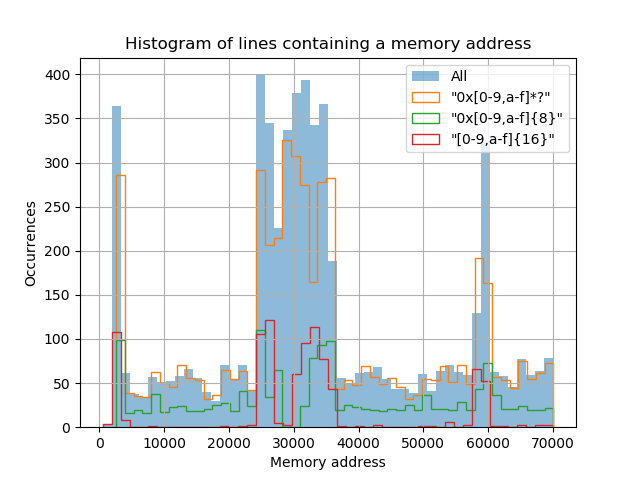
\includegraphics[width=.25\textwidth]{parts/appendix/reports-papud/2018_07_18-Performance_spike_analysis/memory.png}\tabularnewline
Kernel process & 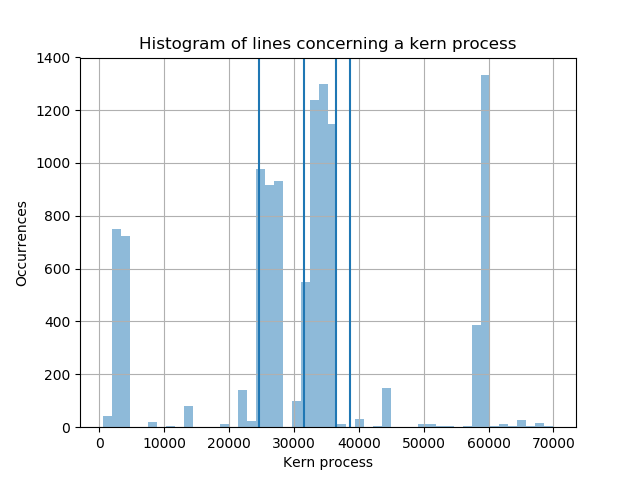
\includegraphics[width=.25\textwidth]{parts/appendix/reports-papud/2018_07_18-Performance_spike_analysis/kern_.png} &
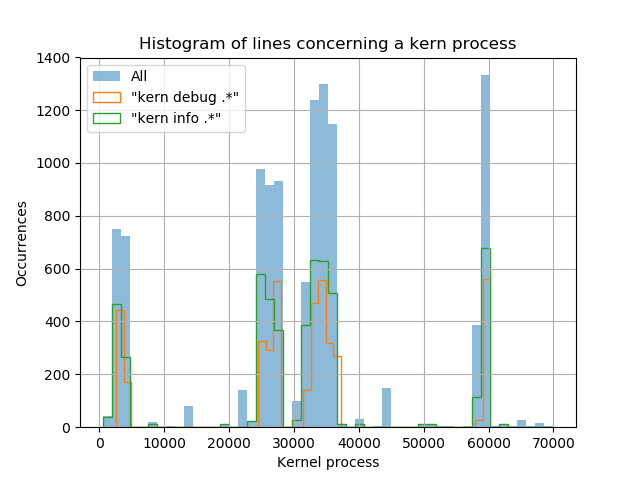
\includegraphics[width=.25\textwidth]{parts/appendix/reports-papud/2018_07_18-Performance_spike_analysis/kern.png}\tabularnewline
Daemon process & 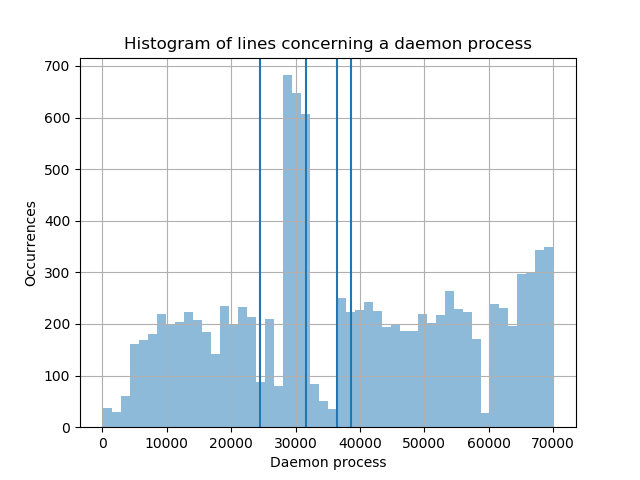
\includegraphics[width=.25\textwidth]{parts/appendix/reports-papud/2018_07_18-Performance_spike_analysis/daemon_.png} &
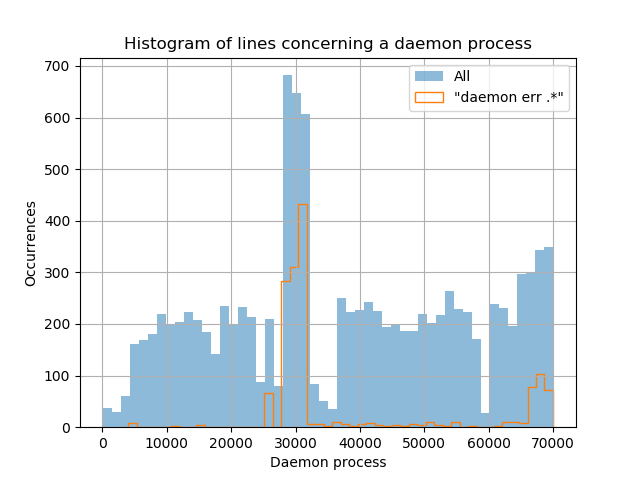
\includegraphics[width=.25\textwidth]{parts/appendix/reports-papud/2018_07_18-Performance_spike_analysis/daemon.png}\tabularnewline
All types & & 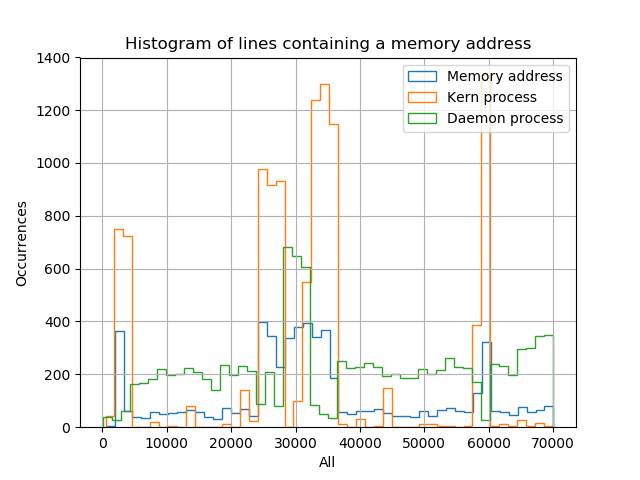
\includegraphics[width=.25\textwidth]{parts/appendix/reports-papud/2018_07_18-Performance_spike_analysis/all.png}\tabularnewline
\hline
\end{longtable}

\subsubsection{Percentages of match in each part of the
corpus}

Percentages of match are percentages on the total line number of the
part of the corpus analysed.

\begin{lstlisting}
--- spike up slope (lines 24545 to 31558, 35% to 45%) ---
Total lines:  7013
Matching "kern .*": 2888 (41%)
Matching "kern info .*": 1458 (20%)
Matching "kern debug .*": 1172 (16%)
Matching "daemon .*": 2048 (29%)
Matching "daemon err .*": 935 (13%)
Matching any memory pattern: 1728 (24%)
Matching "0x[0-9,a-f]{8}": : 196 (2%)
Matching "[0-9,a-f]{16}": : 250 (3%)
Matching "0x[0-9,a-f]*?": : 1478 (21%)

--- spike flat (lines 31558 to 36468, 45% to 52%) ---
Total lines:  4910
Matching "kern .*": 4218 (85%)
Matching "kern info .*": 2154 (43%)
Matching "kern debug .*": 1760 (35%)
Matching "daemon .*": 346 (7%)
Matching "daemon err .*": 174 (3%)
Matching any memory pattern: 1149 (23%)
Matching "0x[0-9,a-f]{8}": : 294 (5%)
Matching "[0-9,a-f]{16}": : 296 (6%)
Matching "0x[0-9,a-f]*?": : 853 (17%)

--- spike down slope (lines 36468 to 38572, 52% to 55%) ---
Total lines:  2104
Matching "kern .*": 27 (1%)
Matching "kern info .*": 15 (0%)
Matching "kern debug .*": 0 (0%)
Matching "daemon .*": 383 (18%)
Matching "daemon err .*": 15 (0%)
Matching any memory pattern: 90 (4%)
Matching "0x[0-9,a-f]{8}": : 34 (1%)
Matching "[0-9,a-f]{16}": : 5 (0%)
Matching "0x[0-9,a-f]*?": : 85 (4%)

--- whole spike (lines 24545 to 38572, 35% to 55%) ---
Total lines:  14027
Matching "kern .*": 7133 (50%)
Matching "kern info .*": 3627 (25%)
Matching "kern debug .*": 2932 (20%)
Matching "daemon .*": 2777 (19%)
Matching "daemon err .*": 1124 (8%)
Matching any memory pattern: 2967 (21%)
Matching "0x[0-9,a-f]{8}": : 524 (3%)
Matching "[0-9,a-f]{16}": : 551 (3%)
Matching "0x[0-9,a-f]*?": : 2416 (17%)

--- full corpus ---
Total lines:  70131
Matching "kern .*": 10972 (15%)
Matching "kern info .*": 5298 (7%)
Matching "kern debug .*": 4134 (5%)
Matching "daemon .*": 10828 (15%)
Matching "daemon err .*": 1504 (2%)
Matching any memory pattern: 5859 (8%)
Matching "0x[0-9,a-f]{8}": : 1586 (2%)
Matching "[0-9,a-f]{16}": : 893 (1%)
Matching "0x[0-9,a-f]*?": : 4987 (7%)

Matching "kern .*" outside of spike: 3839 (5%)
\end{lstlisting}

\subsection{Conclusion(s)}

There are two possible conclusions:
\begin{itemize}
\item the kernel messages are the cause of the spike;
\item or the memory addresses and hexadecimal codes are the cause of the spike.
\end{itemize}

\subsubsection{Kernel messages}

If the kernel messages are the cause of the spike, the most likely
explanation is that this part of the corpus represent a crash of the
server or a major error. In that case, we must remove that part of the
corpus from the training set, as it is not the ``normal'' evolution of
the log.

\subsubsection{Memory addresses and hexadecimal codes}

If the memory addresses and hexadecimal codes are the cause of the
spike, it should be because a succession of number is a very specific
thing to learn. In that case, either we let the model learn the brute
codes, or we replace every code by a ``<hex>'' character to ease the learning
process. It is also possible to replace the different kind of code by a
different character.

\subsection{Improvements and next steps}

To check whether the memory addresses and hexadecimal codes, or the
kernel messages are the cause of the spike, trying to train the model
while replacing every code by a ``<hex>'' character. If there is no
improvement, then the codes are not the cause of the performance spike.

\end{report}
\begin{report}{Rapport de la réunion avec les autres membres du projet}
\section*{Team meeting report}

2018/07/20 - SYNALP - Esteban MARQUER

\subsection{Main points}

\begin{itemize}
\item
  Performance spike issue: see report
  ``2018\_07\_18-Performance\_spike\_analysis''

  \begin{itemize}
  \item
    solution chosen: replace hexadecimal codes with a special label per
    kind of code
  \end{itemize}
\item
  Long training: no over-fitting, 90\% accuracy in 500 epochs

  \begin{longtable}[]{@{}ll@{}}
  \hline
  sequence by sequence mesure & epoch summary\tabularnewline
  \hline
  \endhead
  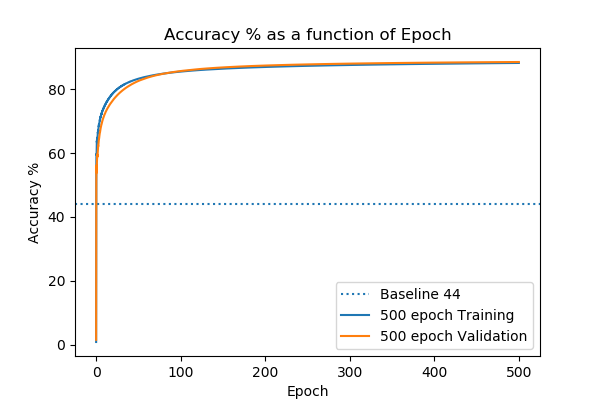
\includegraphics[width=.45\textwidth]{parts/appendix/reports-papud/2018_07_20-500_epochs/accuracy.png} &
  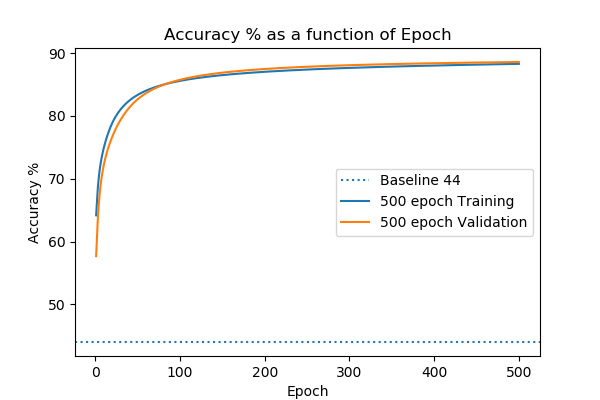
\includegraphics[width=.45\textwidth]{parts/appendix/reports-papud/2018_07_20-500_epochs/accuracy_epoch.png}\tabularnewline
  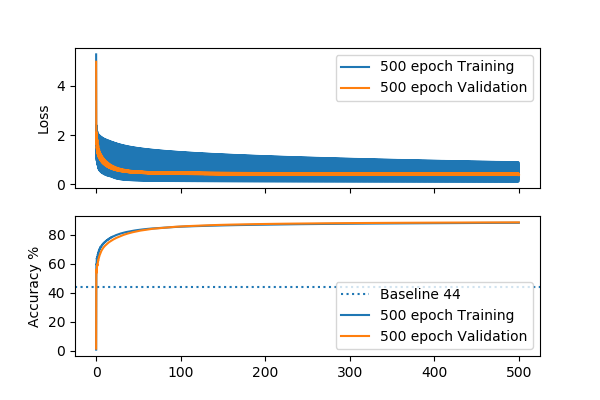
\includegraphics[width=.45\textwidth]{parts/appendix/reports-papud/2018_07_20-500_epochs/loss.png} &
  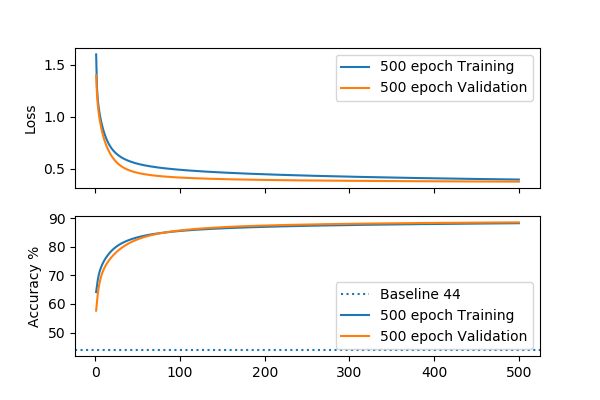
\includegraphics[width=.45\textwidth]{parts/appendix/reports-papud/2018_07_20-500_epochs/loss_epoch.png}\tabularnewline
  \hline
  \end{longtable}
\item
  Baseline accuracy: see first section of ``General\_information.md''
  for values.

  \begin{itemize}
  \item
    Baseline accuracy is high with padding (about 50\%), perhaps lines
    are too long (a lot of padding is needed)
  \item
    Compared with performance, performance is still good
  \end{itemize}
\item
  GPU usage with compleetely loaded corpus: 30\% to 60\%

  \begin{itemize}
  \item
    This is bad new, with such a model training should go at 99\% al the
    time
  \item
    It is necessary to locate the element slowing the process, try
    removing all unecessary processes (logging, storage in memory,
    accuracy, \ldots{})
  \end{itemize}
\item
  New corpus implementation (with buffer and iterators): about
  180s/epoch, 65s/epoch with old implementation (everything loaded in
  memory)

  \begin{itemize}
  \item
    a good implementation of the data loading is critical
  \item
    perhaps pre-loading is too slow because of computations, a
    pre-processed version could help
  \item
    training the model multiple time on a loaded segment could bridge
    the gap between the two processes used
  \item
    using more processes could do the trick (one for loading only, one
    for processing, and one for training)
  \item
    using ``binary''-sized batches (like 8, 64 or 1024) is said to
    achieve faster results, maybe a bit of speed can be gained there
  \end{itemize}
\item
  Development of a learning rate optimisation script: good, better if
  offline (good if both online and offline)

  \begin{itemize}
  \item
    online stands for optimisation before, or/and during every training
  \item
    offline stands for an analysis done a single time, aside from any
    training
  \end{itemize}
\end{itemize}

\subsection{Improvements and next
steps}

\begin{itemize}
\item
  Finish the development of learning rate optimisation.
\item
  Try to make the corpus implementation clean and fast enough (with
  compared run times).
\item
  Integrate the modifications of the corpus processing (memory address
  management)
\item
  Use ``binary''-sized batches; 128 seems perfect, as it is between 50
  and 200 (the bounds found when optimising batches).
\end{itemize}

\end{report}
\begin{report}{Optimisation du taux d'apprentissage}
\section*{Learning rate optimisation}

2018/07/23 - SYNALP - Esteban MARQUER

\subsection{General information}

Learning rate is an hyperparameter in the training algorithm which
changes the speed of the training and the performance of the model.
Specifically, it is a coefficient of the gradient used to update the
parameters of the model.

There are three main learning rates for a model:
\begin{itemize}
\item a learning rate that is too small (closer to 0): the training is slow, and can get blocked in some local minima;
\item a learning rate that is too high (closer to +infinity, usually closer to 1): the learning is faster and avoid local minima, but could diverge from the solution;
\item a balanced learning rate: what we want to find, the traing is fast yet does not diverge.
\end{itemize}

\subsection{Optimisation process}

Usually, learning rate optimisation is done with a logarithmic scale of
the learning rate. The shape of the produced curves confirm the use of
such a scale.

The optimisation process is driven by three parameters and a single
metric.

The metric is the accuracy of the model on the validation corpus at the
end of the training.

The parameters are: the two bounds of the learning rate, and the
learning rate variation factor: the ``learning rate multiplier''.

The learning rate varies as follow in the psedo-python algorythm:

\begin{lstlisting}[language=Python]
# the learning rate takes the highest value as start value, as it will decrease over time
learning_rate = start_value 

# until the learning rate as reach the stop value (the lowest of the two bounds), we make it vary logarithmically
while learning_rate > stop_value:
    performance = train_model(learning_rate)
    save_model_performance(performance, learning_rate)
    
    # the learning rate is updated
    # example with a learning rate of 1 and a learning rate multiplier of 0.1:
    # at first the learning rate is 1, then 0.1, then 0.01 ...
    learning_rate = learning_rate * learning_rate_multiplier

# we compare the performance of the model with the different learning rates
compare_model_performance()
\end{lstlisting}

The closer to 0 the learning rate multiplier is, the faster the
variation will be, and the closer to 1 it si, the slower the variation
will be. To have a decent resolution in the curves, a multiplier close
to 1 is crucial.

The training is done each time on a full epoch.

\subsection{Results}

The first plot is done with a learning rate between 1 and 10\^{}(-5),
with a multiplier of 0.2. The second one is done with a learning rate
between 1 and 10\^{}(-2), with a multiplier of 0.6 (the total of dots is
10).

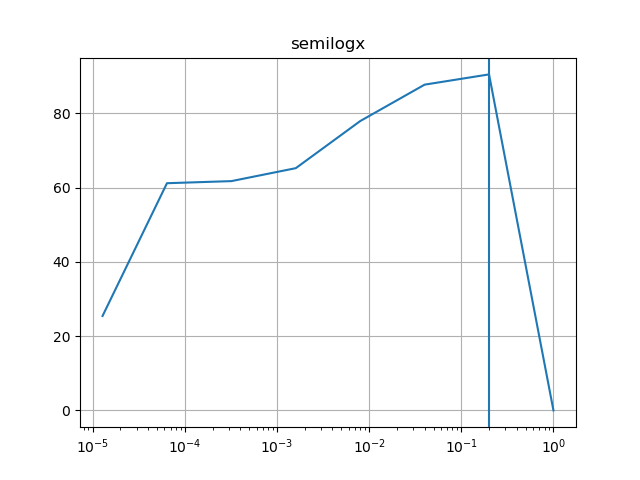
\includegraphics{parts/appendix/reports-papud/2018_07_23-Learning_rate_optimisation/lr_epoch_1_mul_0_2.png}
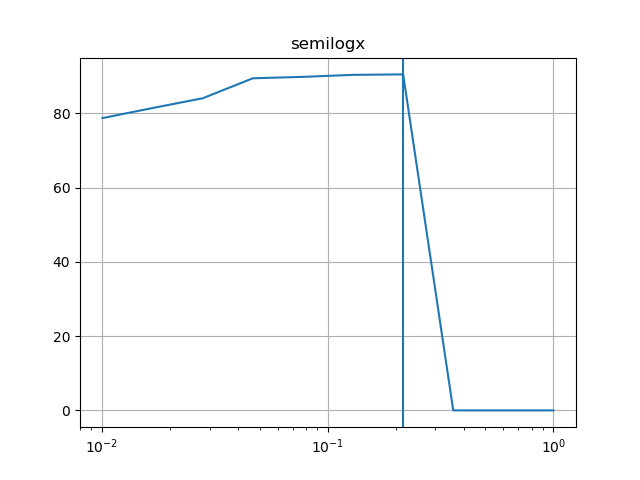
\includegraphics{parts/appendix/reports-papud/2018_07_23-Learning_rate_optimisation/lr_epoch_1_mul_0_6_best_0_216.png}

There is a strange accuracy at the end of the first plot: the
theoretically unreachable 0\%. It is confirmed by the second plot, with
multiple points having an accuracy of 0\%. With a baseline accuracy of
44\%, it is clear that the result diverge from wat is expected. It is a
case of divergence due to a learning rate that is too high.

The best learning rate found is 0.216 (0.6\^{}3), giving the fastest
learning (over 90\% of accuracy in 1 epoch) without diverging.

\subsection{Additional information}

The current implementation consist of a script building a model, and
finding the ideal learning rate for this model. It is an offline
implementation of the model.

The way it is implemented is ideal for an online use too, as the only
operation needed are the removal of the plotting part, and adding the
reload of the model with an updated learning rate.

\subsection{Improvements and next
steps}

Use the new learning rate in the training. As it is quite close to
diverge, it would be advised to use a slightly lower learning rate like
0.2.

If inline optimisation is used, three possibilities seem viable: -
choosing the learning rate every time we start a training, to adapt to
the current hyperparameters; - updating the learning rate every set
number of epochs, to adapt the learning to the current state of the
model; - doing each epoch with a set of learning rates, and every time
choosing the best result; even if costly (every epoch is done multiple
time), it should allow a really fast learning with lowered chances of
divergence or over-fitting.

Personally, my preferred option is the second one.

\end{report}
\begin{report}{Effets de l'optimisation du taux d'apprentissage}
\section*{Learning rate optimisation effect on learning
curve}

2018/07/24 - SYNALP - Esteban MARQUER

\subsection{Context}

The previous results of learning rate optimisation lead to a potentially
optimal learning rate of 0.2 (instead of 0.001).

A run with the new learning rate and every other thing identical was
done to compare performance to previous 500 epoch run. That specific run
had a learning rate of 0.001.

\subsection{Results}

The new learning rate has two effects: 1. convergence is achieved in
less than 100 epoch, compared to previous learning achieving convergence
in more than 400 epochs; 2. a small but constant gap between training
performance and validation performance, but it is not over-fitting (if
both training and validation are constant, we can not conclude that the
model over-fits).

\begin{figure}[ht]
\centering
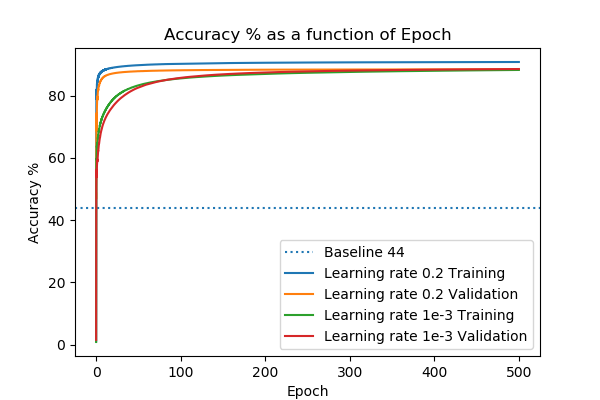
\includegraphics{parts/appendix/reports-papud/2018_07_24-Learning_rate_optimisation_effect/accuracy.png}
\caption{accuracy}
\end{figure}

\subsection{Conclusion}

The new learning rate is better than the previous one, it will be kept.

\subsection{Improvements and next
steps}

{[}OPTIONAL{]} Use inline optimisation to update the learning rate every
set number of epochs (once convergence is reached).

\end{report}
\begin{report}{Taille de \foreign{batch} binaire}
\section*{Binary batch size effect on run
speed}

2018/07/26 - SYNALP - Esteban MARQUER

\subsection{Context}

It has been said that batches using binary sizes (64, 256, 1024,
\ldots{}) perform faster than non-binary sises.

\subsection{Paradigm}

To verify this phenomenon and perhaps improve the training speed, a
comparative experiment has been done with a batch size of 128 and a
batch size of 200.

\subsection{Results}

There is notable no effect, except the effect predicted by the batch
size comparision done previously, and stating that batches with a size
of 200 are faster than with a size of 128.

\begin{figure}[ht]
\centering
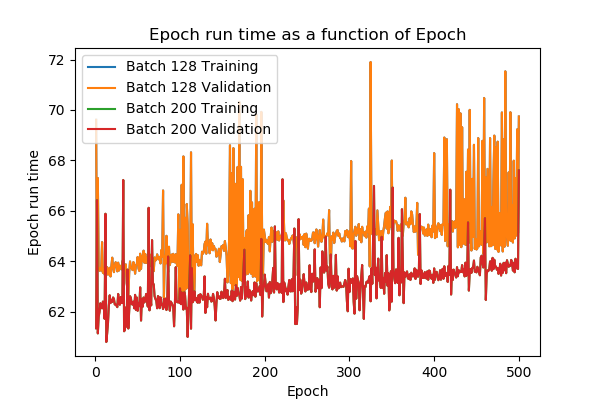
\includegraphics{parts/appendix/reports-papud/2018_07_26-Binary_batch_size/time_epoch.png}
\caption{time per epoch}
\end{figure}

\subsection{Conclusion}

The most straightforward conclusion is that either the effect of binary
sizes is negligible if not non-existent, or there is a hidden parameter
changing th true size of the data (for example a set of bytes used to
store metadata together with the regular data).

As the previous batch size (200) performs better, we will keep it.

\subsection{Next steps and
improvements}

Investigating a potentially non-existent effect (at least with the
current model) does not seem efficient considering the potential gain in
computation time (compared to improving the naive model).

No further work will be done on that now (at least for now).

\end{report}
\begin{report}{Performances du lecteru de corpus multi-fichiers multi-processus}
\section*{Learning rate optimisation effect
on}

2018/07/26 - SYNALP - Esteban MARQUER

\subsection{Context}

Given the large amount of data to process, and the way it is structured
in many small archives, a way to load and pre-process them efficiently
had to be implemented.

\subsection{Multi-file-multi-process corpus
concept}

\subsubsection{Multi-process system}

To avoid the need to completely pre-processing the data and storing it,
and to shift the computational weight of the loading process, the
different tasks are splitted between multipple processes.

At first, the idea was to use three processes, with one for the loading,
one for the pre-processing, and the lat one for the transformation into
tensor. All those process fetch data from a multiprocess-safe queue and
store the result in an output queue, used by the next process as an
input.

A representation of the initial concept:

\begin{lstlisting}
HDD -> Loader -> [raw data queue]
    -> Processing -> [processed data queue]
    -> Tensorising -> [tensors queue]
    -> model
\end{lstlisting}

Given the performance of that system, the slowest part was the
processing. Moreover, the processing could be splitted in multiple
modules: removing the end-of-line characters, replacing paterns by tags
and splitting into characters, transforming the data via a dictionary,
and padding/cropping the sequence.

A representation of the modular processing concept:

\begin{lstlisting}
HDD -> Loader -> [raw Q.]
    -> Process 1 -> [partially processed Q. 1]
    -> Process 2 -> [partially processed Q. 2]
    ...
    -> Process n -> [processed Q. n]
    -> Tensorising -> [tensors queue]
    -> model
\end{lstlisting}

This architecture allows to change the order of the pre-processing
modules, and to add or remove some of them.

By splitting those different tasks on multipple processes, an efficient
processing is achieved. Moreover, it is way easier to add pre-processing
steps.

\subsubsection{Multi-file system}

By considering a set of files as a single sequence of line, and by
loading only the one file containing the current data, combined by
efficient line-by-line sequential reading, a light and fast loading is
achieved.

\subsection{Tests}

\subsubsection{Paradigm}

While setting up the unitary tests for the corpus implementations, three
main situations have produced useful insight on the performances of the
new implementations.

Everything was run on my laptop, with other processes running that may
have hindered the performance (for example, a heavy IDE).

Process-specific tests were run after every element was proven to do
their expected job. Those tests added the processes and the data queues
and information on queue filling and process state.

\subsubsection{Results}

Multiple test were done with very light, light treatment of the data,
and real-situation training (the training is a way to process the data).

\paragraph{Printing only the status of the process at each
batch}

Total time per epoch 12 s

\begin{lstlisting}[language=Python]
{'example': '28032/67923',
 'batch': '218/527',
 'iterator status':
   'Process MultiFile status: process: alive; output queue: 1023/1024
    Process EndLine status: process: alive; output queue: 1023/1024
    Process Regex status: process: alive; output queue: 1024/1024
    Process Dictionary status: process: alive; output queue: 2/1024
    Process CropPad status: process: alive; output queue: 10/1024
    Process Batch status: process: alive; output queue: 0/32'}
\end{lstlisting}

\newpage
\paragraph{Printing the status of the process at each batch and printing
the
data}

Total time per epoch 47 s

\begin{lstlisting}[language=Python]
{'example': '30208/67923',
 'batch': '235/527',
 'iterator status': 
   'Process MultiFile status: process: alive; output queue: 1024/1024
    Process EndLine status: process: alive; output queue: 1024/1024
    Process Regex status: process: alive; output queue: 1023/1024
    Process Dictionary status: process: alive; output queue: 916/1024
    Process CropPad status: process: alive; output queue: 1024/1024
    Process Batch status: process: alive; output queue: 32/32'}
\end{lstlisting}

\paragraph{Printing the status of the process at each batch and training
the
model}

Total time per epoch about 300 s, the old implementation needed about
200 s with the corpus full loaded in GPU RAM. CPU usage (usage mainly by
the program sub-processes): from 60\% to 100\%

\begin{lstlisting}[language=Python]
{'example': '26800/67923',
 'batch': '134/338',
 'iterator status':
   'Process MultiFile status: process: alive; output queue: 1024/1024
    Process EndLine status: process: alive; output queue: 1022/1024
    Process Regex status: process: alive; output queue: 1017/1024
    Process Dictionary status: process: alive; output queue: 905/1024
    Process CropPad status: process: alive; output queue: 975/1024
    Process Batch status: process: alive; output queue: 64/64'}
\end{lstlisting}

\subsection{Conclusions}

The first test shows the without processing the data, we can find where
the data is ``blocked'', and so find the slowest process in the bunch.
Here, the slowest process is the transformation into ids.

As it is a simple dicitonnary reading, which is already a very fast
process in Python, if it is the slowest process of the chain, we can
conclude that the basic performance of this implementation is very good.

When we do even a tyny bit of processing (like printing the data), the
data is blocked at the end of the chain, meaning the printing process is
slower than the loading/pre-processing/tensorising process.

In a true training situation, we can confirm that processing the data is
slower than pre-processing it. The only process slowing the whole
training is the transfer to GPU RAM, which is not in a separate process
yet (due to specificities of pytorch tensor mangement).

The implementation produce equivalent results with multipple files.

Globally, this new implementation should be enough to load and
preprocess the data for the model, vith both small and large datasets.

\subsection{Next steps and
improvements}

\begin{itemize}
\item
  It should be possible to delegate the transfer to GPU RAM to a
  specific process (given the explanations on pytorch manual). This
  should reduce the gap between the speed achieved with pre-loaded data
  andthe speed of the new corpus system.
\item
  The direct next step is to test the new corpus implementation on the
  computer cluster.
\item
  Then, changing the current small corpus by a larger multi-file corpus
  will be possible.
\end{itemize}

\end{report}
